\documentclass[border=3pt]{standalone}
\usepackage{giambattista}
\usepackage{mathmacros} 
\usepackage[svgnames]{xcolor} 
\usepackage[utf8]{inputenc} 
\usepackage{fullpage}
\usepackage{tikz}
\usetikzlibrary{arrows,calc, 
                shapes,positioning}
                
\setmainfont{Latin Modern Sans}
\setmonofont{Cavalcade Mono}
                
\thispagestyle{empty}
\begin{document}
 
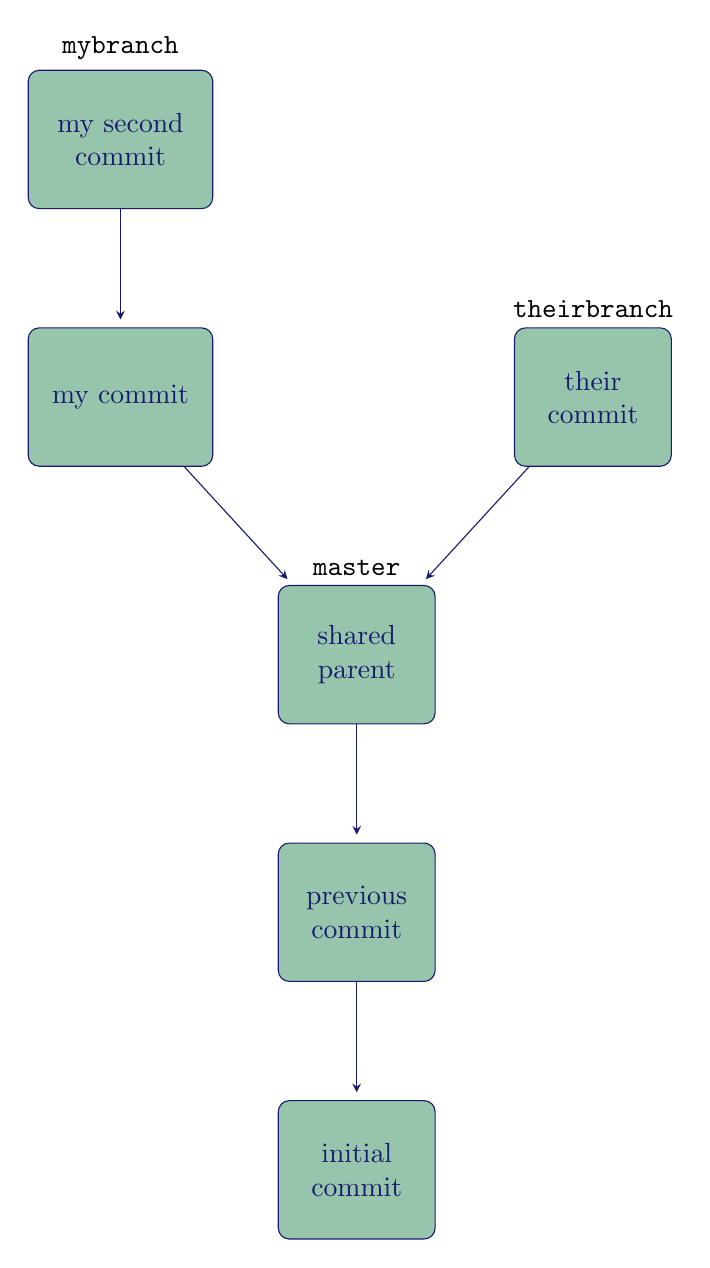
\begin{tikzpicture}
  \tikzset{SectionNode/.style = {shape = rectangle, rounded corners, fill opacity = 0.5, fill = SeaGreen, draw = MidnightBlue, text = MidnightBlue, text opacity = 1, minimum size = 18, minimum height = 50}};
  \tikzset{EdgeStyle/.style = {>=stealth,
      MidnightBlue,text = MidnightBlue,shorten >=1mm,->}};
      
  \node[SectionNode, text width = 50, align = center, label={\texttt{master}}] (shared parent) {shared parent};
  \node[SectionNode, text width = 60, above = 15mm of shared parent, align = center, xshift = -30mm] (my commit) {my commit};
  \node[SectionNode, text width = 60, above = 15mm of my commit, align = center, label={\texttt{mybranch}}] (my second commit) {my second commit};
  \node[SectionNode, above = 15mm of shared parent, text width = 50, align = center, xshift = 30mm, label={\texttt{theirbranch}}] (their commit) {their commit};  
  \node[SectionNode, below = 15mm of shared parent,text width = 50, align = center] (previous commit) {previous commit};
  \node[SectionNode, below = 15mm of previous commit,text width = 50, align = center] (initial commit) {initial commit}; 
  
  \draw[EdgeStyle] (my commit) to (shared parent);
  \draw[EdgeStyle] (their commit) to (shared parent);
  \draw[EdgeStyle] (shared parent) to (previous commit);
  \draw[EdgeStyle] (previous commit) to (initial commit);
  \draw[EdgeStyle] (my second commit) to (my commit);
\end{tikzpicture}
\end{document}